% Intended LaTeX compiler: pdflatex
\documentclass[10pt,a4paper,UTF8]{article}
\usepackage{zclorg}
\usepackage{tikztheorem}
\author{zcl.space}
\date{}
\title{几何分布}
\hypersetup{
 pdfauthor={zcl.space},
 pdftitle={几何分布},
 pdfkeywords={probability},
 pdfsubject={},
 pdfcreator={Emacs 25.0.50.1 (Org mode 9.0.6)},
 pdflang={English}}
\begin{document}

\maketitle
\tableofcontents
\titlepic{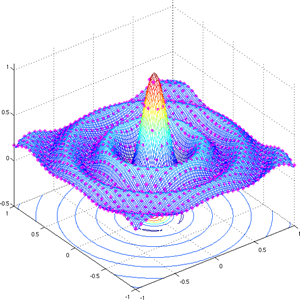
\includegraphics[scale=0.25]{../../img/sinc.PNG}}

\section{几何随机变量}
\label{sec:orgba1f81b}


考虑独立重复试验,每次成功的概率为\(p,0 < p < 1\),重复试验直到试验首次成功为止。如果令\(X\)表示需要试验的次数,那么:
\begin{equation}
\label{eq:1}
P\{X=n\} = (1-p)^{n-1}p,\qquad n = 1,2,\ldots
\end{equation}
由于:
\begin{equation}
\label{eq:2}
\sum_{n=1}^{\infty} P\{X=n\} = p \sum_{n=1}^{\infty} ( 1-p)^{n-1} = \frac{p}{1-(1-p)} = 1
\end{equation}
这说明最终会成功的概率是\(1\),若随机变量的分布列由 (\ref{eq:1})给出,则称该随机变量是参数为\(p\)的几何随机变量。
\section{几何随机变量的期望和方差}
\label{sec:org48724a6}


首先我们计算几何随机变量的期望,令\(q = 1-p\),有:
\begin{eqnarray}
\label{eq:3}
E[X]&=& \sum_{i=1}^{\infty} iq^{i-1}p \\
&=& \sum_{i=1}^{\infty}(i-1+1)q^{i-1}p \\
&=&\sum_{i=1}^{\infty}(i-1)q^{i-1}p + \sum_{i=1}^{\infty} q^{i-1}p \\
&=& q\sum_{j=0}^{\infty}jq^{j-1}p + 1\\
&=&qE[X] + 1
\end{eqnarray}
因此:\[E[X] = \frac{1}{p}\]
一个成功概率为\(p\)的试验,如果独立重复进行直到饰演陈宫,那么需要进行的试验的期望次数邓毅\(\tfrac{1}{p}\)。掷一枚均匀的骰子,直到出现一次点数为\(1\),需要的期望次数为\(6\).

然后我们计算几何随机变量的方差。首先计算\(E[X^{2}]\),有:
\begin{eqnarray}
\label{eq:4}
E[X^{2}]&=& \sum_{i=1}^{\infty} i^{2}q^{i-1}p \\
&=&\sum_{i=1}^{\infty} (i-1+1)^{2}q^{i-1}p \\
&=&\sum_{i=1}^{\infty} (i-1)^{2}q^{i-1}p + \sum_{i=1}^{\infty} 2(i-1)q^{i-1}p + \sum_{i=1}^{\infty}q^{i-1}p \\
&=&\sum_{j=0}^{\infty}j^{2}q^{j}p + 2\sum_{j=1}^{\infty}jq^{j}p + 1 \\
&=&qE[X^{2}] + 2qE[X] +1
\end{eqnarray}
结合\(E[X]=1/p\),我们可以得到:
\begin{equation}
\label{eq:5}
pE[X^{2}] = \frac{2q}{p} + 1
\end{equation}
因此:
\begin{equation}
\label{eq:6}
\mathrm{Var}(X) = \frac{q+1}{p^{2}} - \frac{1}{p^{2}} = \frac{q}{p^{2}} = \frac{1-p}{p^{2}}
\end{equation}
\section{一个例子}
\label{sec:orgbc3b044}


每一个概率分布都有其现实中的例子。接下来给出一个几何随机变量的例子。

\begin{tikzproblem}
一个坛子中有\(N\)个白球和\(M\)个黑球,每次从中抽取一个球,观察球的颜色并放回,重复这个过程,直到取出一个黑球,求以下事件的概率:
\begin{enumerate}
\item 恰好取球\(n\)次。
\item 至少取球\(k\)次。
\end{enumerate}
\end{tikzproblem}

\begin{tikzanswer}
如果我们令\(X\)表示要取出一个黑球需要的取球次数,则\(X\)满足 (\ref{eq:1})且\(p=\frac{M}{N+M}\)。所以:
\begin{equation}
\label{eq:7}
P\{X=n\} = (\frac{N}{M+N})^{n-1}\frac{M}{M+N} = \frac{MN^{n-1}}{(M+N)^{n}}
\end{equation}

对于第二个问题,
\begin{equation}
\label{eq:8}
P\{X\geq k\} = \frac{M}{M+N}\sum_{n=k}^{\infty} \bigg( \frac{N}{M+N} \bigg)^{n-1} = \bigg( \frac{N}{M+N} \bigg)^{k-1}
\end{equation}
式 (\ref{eq:8})的结果可以直接得到,因为至少需要\(k\)次取球意味着前\(k-1\)次拿到的都是白球,即前\(k-1\)次试验都失败。故对于一个服从几何分布的随机变量\(X\),有:
\begin{equation}
\label{eq:9}
P\{X\geq k\} = (1-p)^{k-1}
\end{equation}
\end{tikzanswer}
\end{document}
